\RequirePackage{luatex85}


\documentclass{standalone}
\usepackage{tikz} 
%include other needed packages here
\usepackage{tikz-feynman}

\tikzfeynmanset{compat=1.0.0}

\tikzfeynmanset{
  myblob/.style={
  shape=circle,
  draw=red,
  fill=red,
  minimum size=0.35cm,
  scale=0.35,
  text = red,
  }
}

\tikzset{myblob2/.style={
  shape=circle,
  draw=red,
  fill=red,
  minimum size=0.60cm,
  scale=0.60,
  text = red,
  }
  }

\usepackage{graphicx}
\usepackage{caption}
\usepackage{subcaption}

\begin{document}

    \feynmandiagram [horizontal=b to d, spring layout] {
      a [particle=\(q\)] -- [fermion] b [],
      b -- [gluon] c [particle=\(g\)],
      b -- [fermion] d [myblob,label=\({\kappa_{qq'H}}~~~~\)],
      d [particle=\(q'\)] -- [fermion] o2 [particle=\(q'\)],
      d -- [scalar] o1 [particle=\(H\)],
    };


\iffalse
    \feynmandiagram [horizontal=b to d, spring layout] {
      a [particle=\({q'}\)] -- [fermion] b [myblob,label=\({~~~~~~~\kappa_{qq'H}}\)],
      b -- [fermion] c [particle=\(\bar{q}\)],
      d [particle=\(H\)] -- [scalar] b,
      };
\fi 
      
\iffalse
    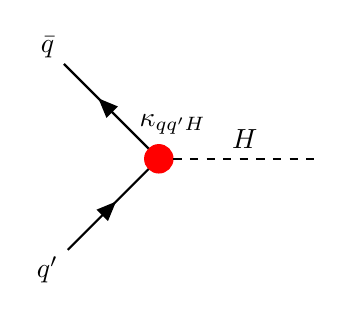
\begin{tikzpicture}[]
      \begin{feynman}[large]
        \vertex                     (i1) { \(\bar{q}\)};
        \vertex [below right      =of i1, myblob2, label=\({~~~\kappa_{qq'H}}\)] (a) {};
        \vertex [right      =of a] (f1)  {};
        \vertex [below left      =of a] (i2) {\(q'\)};
        \vertex [right      =of a] (b);
        
        \diagram* {
          (a) -- [fermion] (i1),
          (a)  -- [scalar,  edge label=\(H\)] (b),
          (i2) -- [fermion] (a),
        };
      \end{feynman}
    \end{tikzpicture}
\fi 

\iffalse
    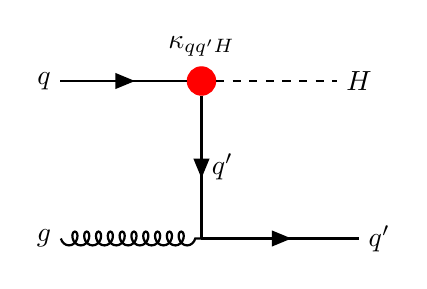
\begin{tikzpicture}[]
      \begin{feynman}[large]
        \vertex                     (i1) { \(q\)};
        \vertex [right      =of i1,myblob2, label=\({\kappa_{qq'H}}\)] (a) {};
        \vertex [right      =of a] (f1)  {\(H\)};
        \vertex [below      =of i1] (i2) {\(g\)};
        \vertex [right      =of i2] (b);
        \vertex [right      =of b] (f2)  {\(q'\)};
        
        \diagram* {
          (i1) -- [fermion] (a) -- [scalar] (f1),
          (a)  -- [fermion,  edge label=\(q'\)] (b),
          (i2) -- [gluon] (b) -- [fermion] (f2),
        };
      \end{feynman}
    \end{tikzpicture}

\fi 

\iffalse
    \feynmandiagram [horizontal=b to d] {
      a [particle=\({q'}\)] -- [fermion] b [myblob,label=\({~~~~~~~\kappa_{qq'H}}\)],
      b -- [fermion] c [particle=\(\bar{q}\)],
      d [particle=\(H\)] -- [scalar] b,
      };
\fi  
      
\iffalse
    \feynmandiagram [inline=(d.base), horizontal=d to b] {
      b [myblob,label=\({ \kappa_{tqg}~~~~~  }\)] -- [fermion] a [particle=\({u,c}\)],
      b -- [gluon] c [particle=\(g\)],
      d [particle=\(t\)] -- [fermion] b,
      };
\fi  

\iffalse
    \feynmandiagram [inline=(d.base), horizontal=d to b] {
      b [myblob,label=\({ \kappa_{tq\gamma}~~~~  }\)] -- [fermion] a [particle=\({u,c}\)],
      b -- [boson] c [particle=\(\gamma\)],
      d [particle=\(t\)] -- [fermion] b,
      };
\fi  

\iffalse
    \feynmandiagram [inline=(d.base), horizontal=d to b] {
      b [myblob,label=\({ X_{tqZ},~\kappa_{tqZ}~~~~~~~~~~~~~~ }\)] -- [fermion] a [particle=\({u,c}\)],
      b -- [boson] c [particle=\(Z^0\)],
      d [particle=\(t\)] -- [fermion] b,
      };
\fi  

\iffalse
    \feynmandiagram [inline=(d.base), horizontal=d to b] {
      b [myblob,label=\({\kappa_{tqH}~~~~  }\)] -- [fermion] a [particle=\({u,c}\)],
      b -- [scalar] c [particle=\(H^0\)],
      d [particle=\(t\)] -- [fermion] b,
      };
\fi  

\end{document}



\iffalse
\documentclass{article}

\usepackage{tikz}
\usepackage{tikz-feynman}
\pgfrealjobname{survey}


\tikzexternalize
\tikzfeynmanset{compat=1.0.0}

\tikzfeynmanset{
  myblob/.style={
  shape=circle,
  draw=black,
  fill=black,
  minimum size=0.25cm,
  scale=0.25
  }
}

\begin{document}
  \beginpgfgraphicnamed{survey-f1}
  \feynmandiagram [inline=(d.base), horizontal=d to b] {
      b [myblob,label=\({ \kappa_{tqg}~~~~~  }\)] -- [fermion] a [particle=\({u,c}\)],
      b -- [gluon] c [particle=\(g\)],
      d [particle=\(t\)] -- [fermion] b,
      };
   \endpgfgraphicnamed
        
\end{document}
\fi

\iffalse
\begin{figure}
  \centering
  \begin{subfigure}[t]{0.24\textwidth}
    \centering
    \feynmandiagram [inline=(d.base), horizontal=d to b] {
      b [myblob,label=\({ \kappa_{tqg}~~~~~  }\)] -- [fermion] a [particle=\({u,c}\)],
      b -- [gluon] c [particle=\(g\)],
      d [particle=\(t\)] -- [fermion] b,
      };
  \end{subfigure}
  \begin{subfigure}[t]{0.24\textwidth}
    \centering
    \feynmandiagram [inline=(d.base), horizontal=d to b] {
      b [myblob,label=\({ \kappa_{tq\gamma}~~~~  }\)] -- [fermion] a [particle=\({u,c}\)],
      b -- [boson] c [particle=\(\gamma\)],
      d [particle=\(t\)] -- [fermion] b,
      };
  \end{subfigure}
  \begin{subfigure}[t]{0.24\textwidth}
    \centering
    \feynmandiagram [inline=(d.base), horizontal=d to b] {
      b [myblob,label=\({ X_{tqZ},~\kappa_{tqZ}~~~~~~~~~~~~~~ }\)] -- [fermion] a [particle=\({u,c}\)],
      b -- [boson] c [particle=\(Z^0\)],
      d [particle=\(t\)] -- [fermion] b,
      };
  \end{subfigure}
  \begin{subfigure}[t]{0.24\textwidth}
    \centering
    \feynmandiagram [inline=(d.base), horizontal=d to b] {
      b [myblob,label=\({\kappa_{tqH}~~~~  }\)] -- [fermion] a [particle=\({u,c}\)],
      b -- [scalar] c [particle=\(H^0\)],
      d [particle=\(t\)] -- [fermion] b,
      };
  \end{subfigure}
  \caption{Diagrams for top quark decays mediated by FCNC couplings.}
  \label{fcnc_decays}       % Give a unique label
\end{figure} 
\fi

